\subsubsection{\texttt{RF-6}: configuración de soluciones para profesores}
\label{subsec:rf6}

Uno de los objetivos principales fijados para la evolución del proyecto es permitir al profesorado adjuntar a los ejercicios su propia propuesta de resolución, que será accesible a los estudiantes una vez sea publicada. Este requisito es uno de los que busca dar cumplimiento al objetivo tercero del \referenciaCapitulo{cap:objetivos}.

El presente requerimiento tiene como fin la incorporación de controles que permitan a los profesores determinar cuándo es pública una solución y si los estudiantes pueden (o no) hacer modificaciones a sus propuestas propias de resolución de los ejercicios una vez hayan accedido a la solución propuesta por el docente.

De este modo, las soluciones permanecen ocultas por defecto a los estudiantes hasta que el profesor decida publicarlas, siendo este cambio irreversible; esto es, una vez publicada no puede ser despublicada. Por otro lado, el comportamiento por defecto de la aplicación es el de bloquear la edición de los ejercicios una vez el estudiante descargue la propuesta de solución del docente, pasándolo a estado ``finalizado'' automáticamente cuando el estudiante inicie la descarga de la solución, previa solicitud de confirmación. Si el docente lo desea, puede modificar este comportamiento, de modo que el estado permanecerá con el valor ``en progreso'' a pesar de haber descargado la solución, considerando que este ajuste debe estar adecuadamente configurado antes de la publicación de la solución, ya que este parámetro también permanecerá inmutable tras publicarla. Ambas modificaciones de configuración se pueden realizar a través del \textit{dashboard} de los ejercicios que tienen solución, tal como se puede apreciar en la \referenciaFigura{fig:reqf6-1}.

Para efectuar esta implementación, se han realizado los siguientes cambios:
\begin{itemize}
    \item Se han alterado los modelos de dominio de la entidad relativa a los ejercicios tanto en el servidor como en el cliente para introducir dos valores \textit{booleanos} para controlar la disponibilidad de la solución y la capacidad de edición tras su descarga.
    \item Se han introducido dos elementos de interacción de usuario en forma de casillas de verificación para dotar al profesorado de la capacidad para modificar los atributos de configuración descritos con anterioridad. Estos elementos quedan señalados en la figura anteriormente referenciada.
\end{itemize}

\begin{figure}[ht]
    \centering
    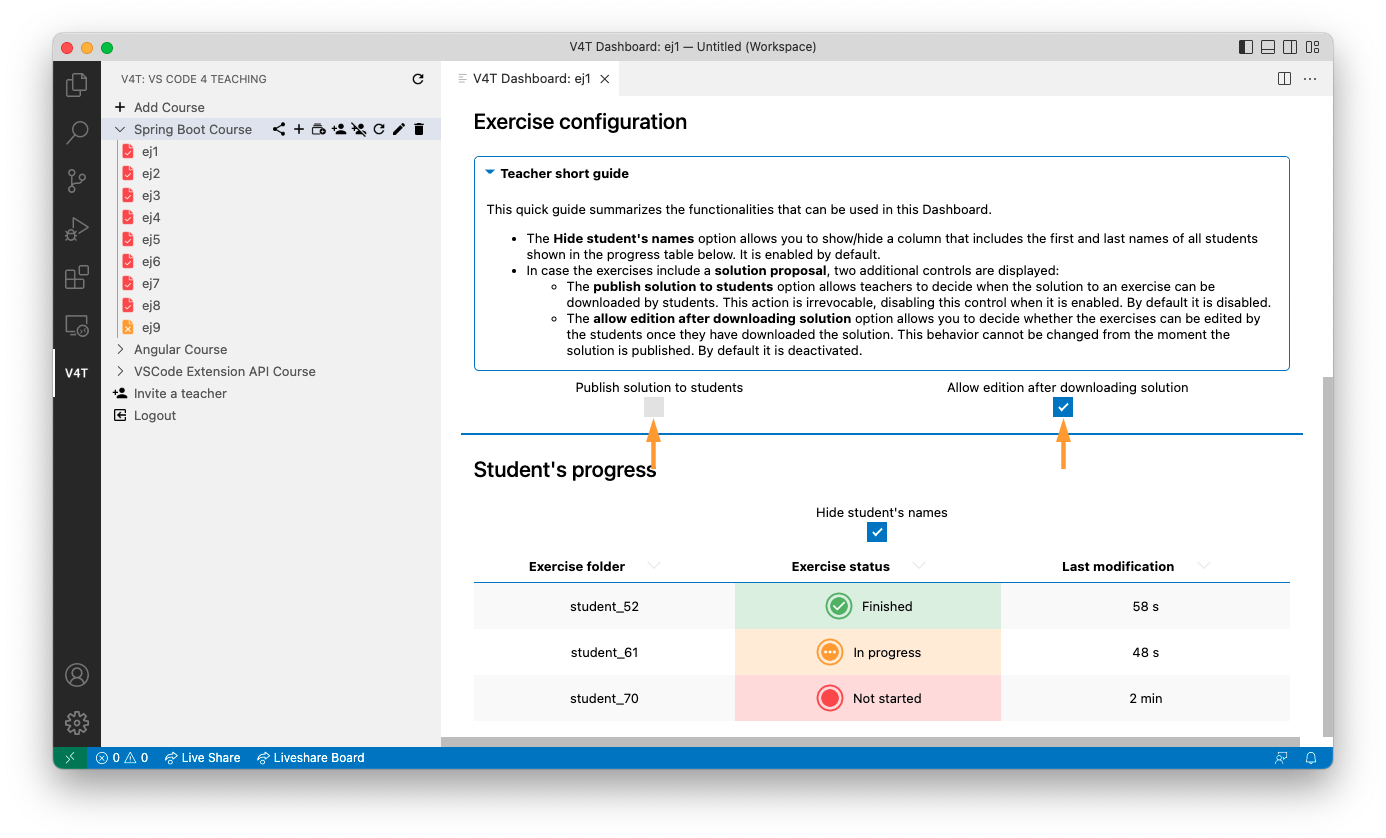
\includegraphics[width=\textwidth]{imagenes/utilizadas/4-3-implementacion/rf6-1.png}
    \caption{Captura de la extensión en la que se destacan los elementos gráficos para la modificación de la configuración de la solución de un ejercicio.}
    \label{fig:reqf6-1}
\end{figure}
